\documentclass[12pt, a4]{article}
\usepackage{blindtext}
\usepackage{graphicx}
\usepackage{subcaption}
\usepackage{float}

\usepackage[margin=0.75in]{geometry}
\graphicspath{{./images/}}

\title{%
Finding the best position of centre of mass of cyclist and bike for most efficient safe braking \\
\large International Baccalureate Extended Essay}
\author{Igor Krzywda}

\begin{document}
\maketitle

\section{Introduction}
\subsection{Context}
Braking is the most important safety feature on a bicycle, however when misused braking can be the cause of the
most severe crashes one can have on a bicycle. Many of such crashes are caused by the lack of understanding of
mechanics of braking a bicycle. There are countless tutorials on how to brake properly on a bicycle, but most of
them are based on empirical experience of more proffesional riders. Such advice falls in line with physical 
analysis, but is mostly biased by many factors spanning from the type of cycling the tutorial is based on to 
the attitude towards crashing of the presenter. There is clearly a void in giving an objective advice on safety 
on a bicycle that can be a base to domain-specific guides.

\subsection{Scope of research}
This essay will be exploring the placement of centre of mass for maximum braking while maintaining safety. 
The analysis will be split into two parts-a theoretical one involving building an universal model for finding 
best braking setup and a practical one, which will serve as a validation of the theoretical model using sensor
data.

\subsection{The goal of the research}
The goal of the research is to create an universal model for finding the best braking position in terms of
centre of mass on any bicycle. Such model will serve as a basis for explaining why it is important to find 
a bike fitting its rider and giving the reader an idea of where the limits of his equipment are without 
finding about it by crashing.

\section{Theoretical analysis of braking a bicycle}
\subsection{Rules and assumptions for the analysis}
Assumptions about bicycle and rider:
\begin{itemize}
\item{rider and bicycle make one rigid body}
\item{there is no dissipation of force}
\end{itemize}
Safe braking in the analysis is defined by two factors:
\begin{itemize}
\item{rear wheel makes contact with the surface at all times}
\item{no wheel is skidding while braking}
\end{itemize}
Neglected factors\footnote[1]{these factors play more significant role in reality than they do in theoretical
considerations}:
\begin{itemize}
\item{decrease in braking power due to heat and brake pad residue}
\item{dynamic change in frame geometry due to amortisation and tire compression}
\item{air drag}
\item{rolling resistance}
\end{itemize}

\subsection{Theoretical model of bicycle and cyclist}
The model of bike and a rider for this analysis is two dimensional, because no lateral forces are taken in 
consideration. The cases for safe braking are checked with the state of wheels, hence the focal point of the 
analysis will be forces excerted on axles, so the whole frame of the bike can be reduced to a single beam 
spanning from axle to axle. The rider is reduced to net centre of mass of bike and cyclist, which is connected
perpendicularly to the virtual beam. Figure~\ref{fig:theoretical_models} shows the simplification of the model.
\begin{figure}[h]
\caption{}
\centering
\begin{subfigure}[b]{0.3\linewidth}
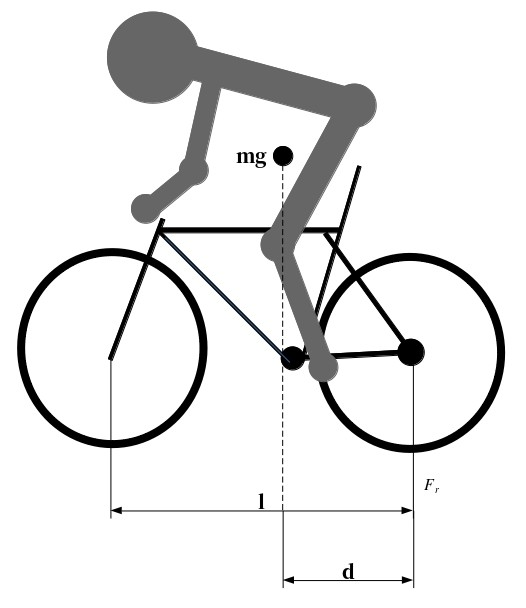
\includegraphics[width=\linewidth]{bike_static_model_bike}%
\label{fig:bike_diagram}
\caption{}
\end{subfigure}
\begin{subfigure}[b]{0.3\linewidth}
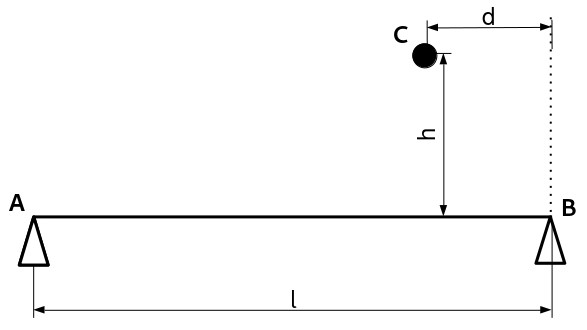
\includegraphics[width=\linewidth]{bike_static_model_simplified}
\caption{}%
\label{fig:beam_diagram}
\end{subfigure}%
\label{fig:theoretical_models}
\end{figure}

\subsection{Force distribution on the axles}
The force distribution on the axles is the most important part of the analysis, as it gives us data to 
determine the deceleration and whether or not the conditions for safe braking are maintained.

\subsubsection{Cyclist static or moving at constant speed}
\begin{figure}[H]
\centering
\caption{}
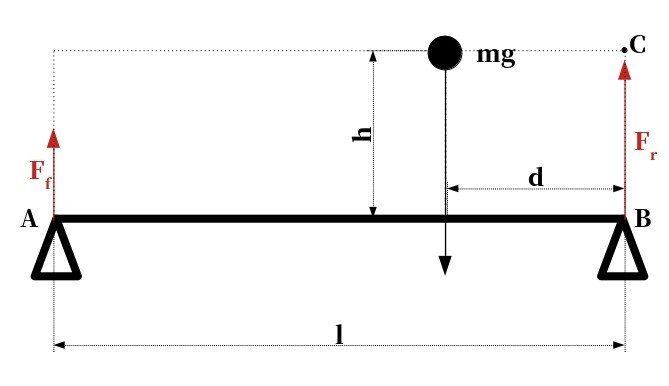
\includegraphics[width=\linewidth]{static_forces_simplified}%
\label{fig:static_diagram}
\end{figure}
First let us consider the case of the cyclist being stationary or moving at a constant speed. In order to 
calculate the forces on each axle, we need to consider moments of force applied to the frame, which will be
our moment arm $l$ (fig.~\ref{fig:static_diagram}). When a cyclist is on the bike, the point on the frame, where
the force is being excerted is right below his centre of mass. In order to calculate the either of the forces 
on the axles, we need to equate internal torques to either point A or B in fig.~\ref{fig:static_diagram}: 
\begin{equation}
\centering%
\label{eq:equating_torques}
F_f \cdot l = mg \cdot d
\end{equation}

From this equation we can derive load on front axle (eq.~\ref{eq:F_f}). The net force on acting 
on the bike is $mg$, therefore the load on rear axle will be described as in equation~\ref{eq:F_r}
\begin{equation}
\centering%
\label{eq:F_f}
F_f = \frac{mg \cdot d}{l}
\end{equation}
\begin{equation}
\centering%
\label{eq:F_r}
F_r = mg - F_f
\end{equation}

\begin{figure}[H]
\centering
\caption{}
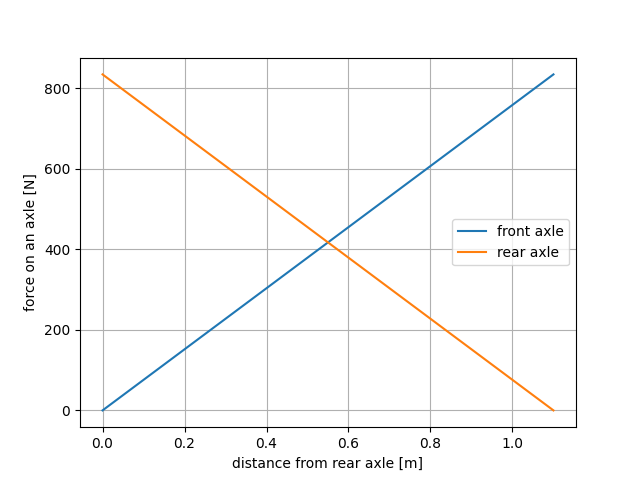
\includegraphics[width=0.5\linewidth]{axles_static_graph}%
\label{fig:static_graph}
\end{figure}
When we plot these equations as functions of the distance, (fig.~\ref{fig:static_graph})\footnote[1]{graph is 
generated with parameters from the experiment}. The load on the front axle is a linear function with 
coefficient of $\frac{mg}{l}$, which means that the heavier the rider and bike, the steeper the graph.
Same effect would have been making the bike shorter. The force on the rear axle is the inverse of front one.

\subsubsection{Cyclist decelerating}
\begin{figure}[H]
\centering
\caption{}
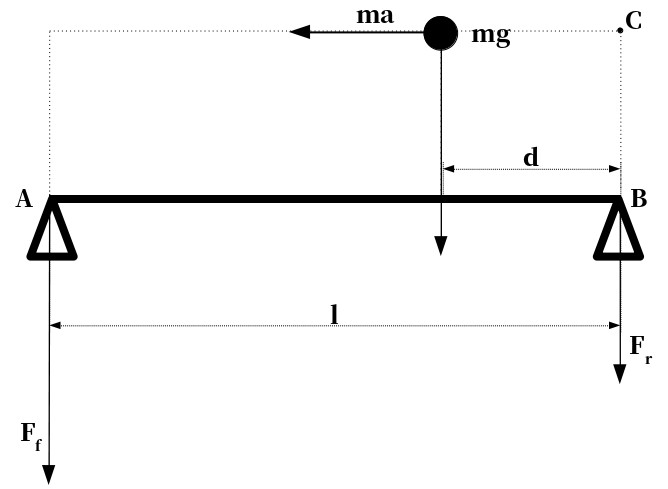
\includegraphics[width=0.5\linewidth]{decelerating_forces_diagram}%
\label{fig:deceleration_diagram}
\end{figure}
For this moment we will consider cyclist just decelerating neglecting what is happening to wheels, focusing
our attention on axles just like in section above. When decelerating, aside from forces caused by the weight, 
we also need to consider force coming from deceleration of the body. From second Newton's law we know that 
$F = ma$, however we are considering our problem in terms of torque, so we need to find the lever arm this
force is acting upon. As mentioned above we are assuming that bicycle and the rider are one rigid body. 
Having assumed that, we can say that the centre of mass of bike and rider is connected with a virtual lever
connected at 90 degrees to our main moment arm, which is the bike frame. Just like before, we need to equate 
the moments, but in this case, we need to equate them to point C, as we need to include vertical lever 
(fig.~\ref{fig:deceleration_diagram}): 
\begin{equation}
\centering%
\label{eq:eq_torques_dyn}
F_f \cdot l = mg \cdot d + ma \cdot h
\end{equation}
And just like in previous example, the force in the rear is: 
\begin{equation}
\centering%
\label{eq:eq_torques_dyn}
F_r = mg - F_f
\end{equation}
In this case, however, it is possible for forces to be negative (fig~\ref{fig:dynamic_graph}).
\begin{figure}[H]
\centering
\caption{}
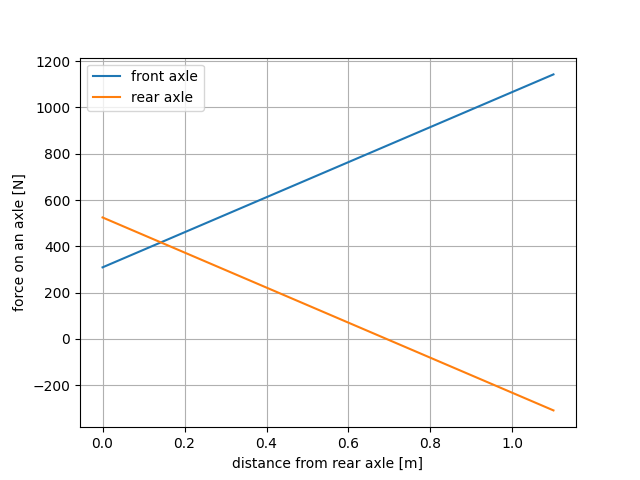
\includegraphics[width=0.6\linewidth]{axles_dynamic_graph}%
\label{fig:dynamic_graph}
\end{figure}

\section{Physical explanation of safe braking}
\subsection{Maintaining rolling of wheels while braking}
\begin{figure}[H]
\centering
\caption{}
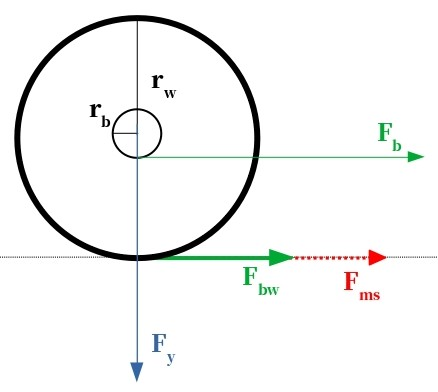
\includegraphics[width=0.5\linewidth]{wheel_braking_forces}%
\label{fig:wheel_diagram_1}
\end{figure}
The limiting factor for braking without skidding is the maximum frictional force between the tire and the 
surface, which is calculated by:
\begin{equation}
\centering%
\label{eq:F_ms}
F_{ms} = F_y \cdot \mu
\end{equation}
When the braking force exceeds the maximum frictional force, the wheel locks up. In order to compare braking 
force with maximum friction, we need to find the braking vector with the same origin as the friction. We do 
that by equating torques to that point like so:
\begin{equation}
\centering%
\label{eq:F_bw}
F_b \cdot r_b = F_{bw} \cdot r_w
\end{equation}
Therefore, from equations~\ref{eq:F_ms} and~\ref{eq:F_bw} we can see that in order to brake and not skid the 
following condition must be met:
\begin{equation}
\centering%
\label{eq:braking_final_eq}
F_y \cdot \mu \geq F_{bw}
\end{equation}
Note that we are referring to the braking force as $F_{bw}$ only. This is because of the abundance of different
types of brakes found on bikes, in order to make the analysis universal we need to look at the output force rather
than the input one, which would be relevant for checking whether the brake would be capable of exceting
such stopping force. The other thing that should be emphasised in equation~\ref{eq:braking_final_eq} is the 
more-or-equal sign. Braking at force equal is very unstable, as smallest spike in force can cause instantaneus 
skidding because of the gap between static and dynamic friction coefficient.

\subsection{Keeping rear wheel from lifing off}
\begin{figure}[H]
\caption{}
\centering%
\label{fig:angular_acceleration_figure}
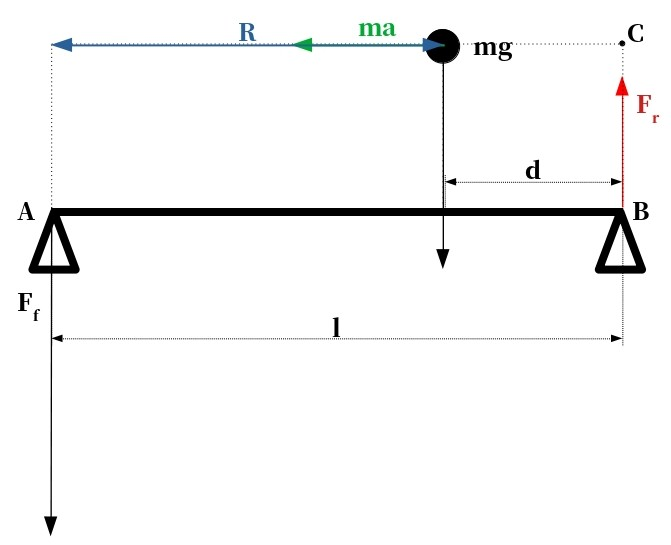
\includegraphics[width=0.5\linewidth]{angular_acceleration_diagram}%
\end{figure}
The more dangerous threat when braking is angular acceleration of the whole bike around the front axle resulting
in rear wheel getting into the air. In order for that to happen, there must be a vector of force pointing upwards
from rear axle, which, as we can see in figure~\ref{fig:dynamic_graph} appears as negative values on the graph.
In order to calculate the angular acceleration ($\alpha$), we need to calculate the moment of inertia of rider 
and bicycle.
\begin{equation}
\centering%
\label{eq:moment_of_inertia}
\sum \tau = F_r \cdot l =  I\alpha = MR^2\alpha
\end{equation}
The sum of torques in our case is the moment excerted by $F_r$ only, as the torque excerted by the $F_f$ is 
zero because its lever arm is 0. Knowing that, $\sum \tau$ can be denoted just as $\tau$. With that, we can
calculate the angular acceleration of the whole body while braking
\begin{equation}
\centering%
\label{eq:angular_acceleration_eq}
\alpha = \frac{\tau}{MR^2}
\end{equation}
If we plot equation~\ref{eq:angular_acceleration_eq} as a function of distance from the rear axle along with 
torque and moment of inertia, we can see just how quickly the angular acceleration rises when the centre of mass
gets closer to the axis of rotation. With this graph we can see that when we get close enough to the axis of 
rotation, every centimeter can have a huge impact on the angular acceleration, and in turn the reaction time 
we have to prevent what is widely known as going over the bars.
\begin{figure}[H]
\caption{}
\centering%
\label{fig:angular_acceleration_graph}
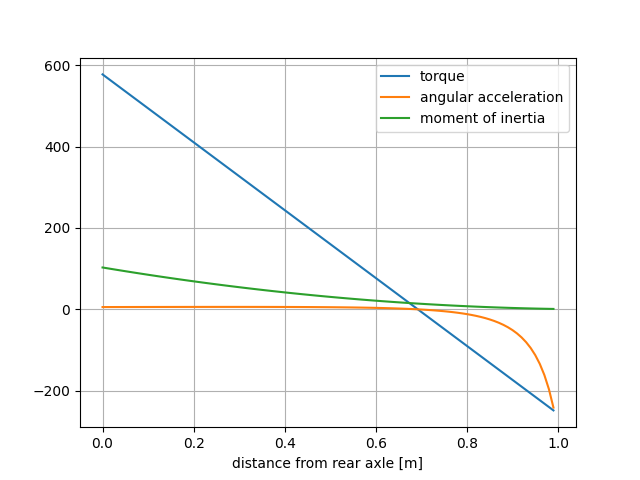
\includegraphics[width=0.8\linewidth]{angular_acceleration}%
\end{figure}

\section{Applying the theoretical model to safety on the bicycle}
When riding a bicycle, our safety is in majority dependent on our skill level rather than on the bicycle itself, 
but knowing the physics standing behind our safety on the bike, we can both increas our safety on the saddle,
as well as even before we choose our machine.
\subsection{Bikefitting}
Bikefitting is a whole industry centered around, as the name suggests, fitting bikes to a person. There are
dedicated businesses as well as calculators, but since there is the issue of relying on experience of a 
proffesional rider and because the calculators are proprietary software, we are unable to understand why we get
the particular frame. Of course bikefitting is much, much broader than just setting up the bike for braking, as there
are different disciplines and types of riding, but in this example we are assuming that we want to optimize our bike
for maximum safety while braking. \\
\begin{figure}[H]
\centering 
\begin{subfigure}[b]{0.45\linewidth}
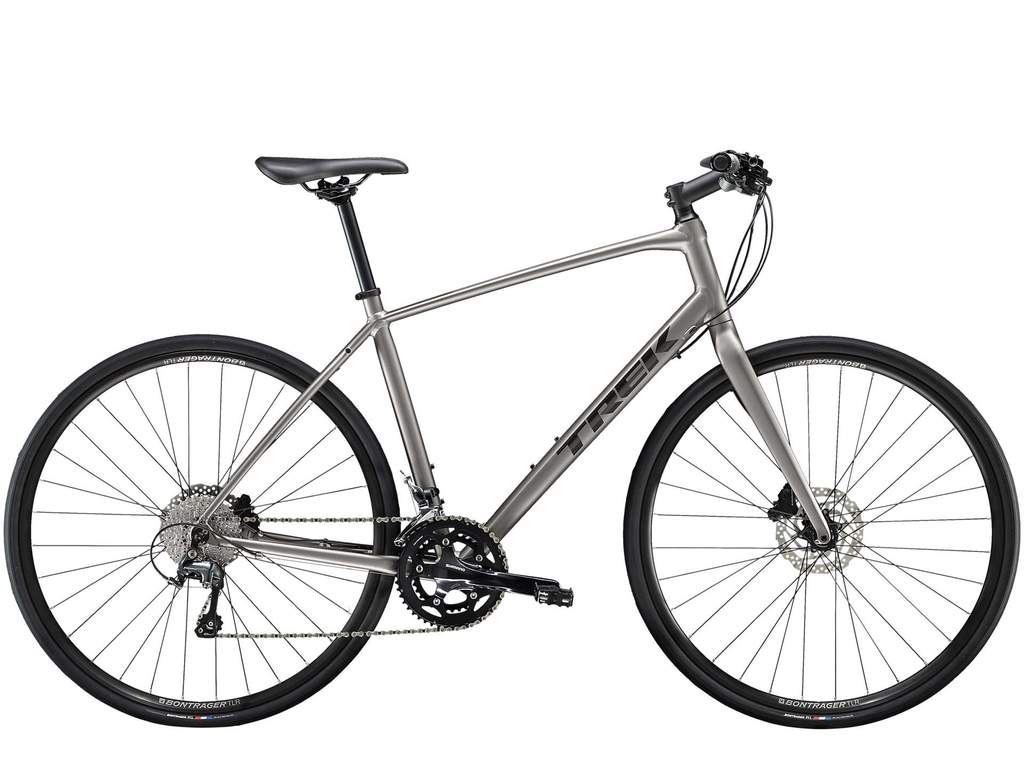
\includegraphics[width=\linewidth]{trek_fx_sport_4}%
\label{fig:trek_fx_sport_4_pic}
\caption{}
\end{subfigure}
\begin{subfigure}[b]{0.45\linewidth}
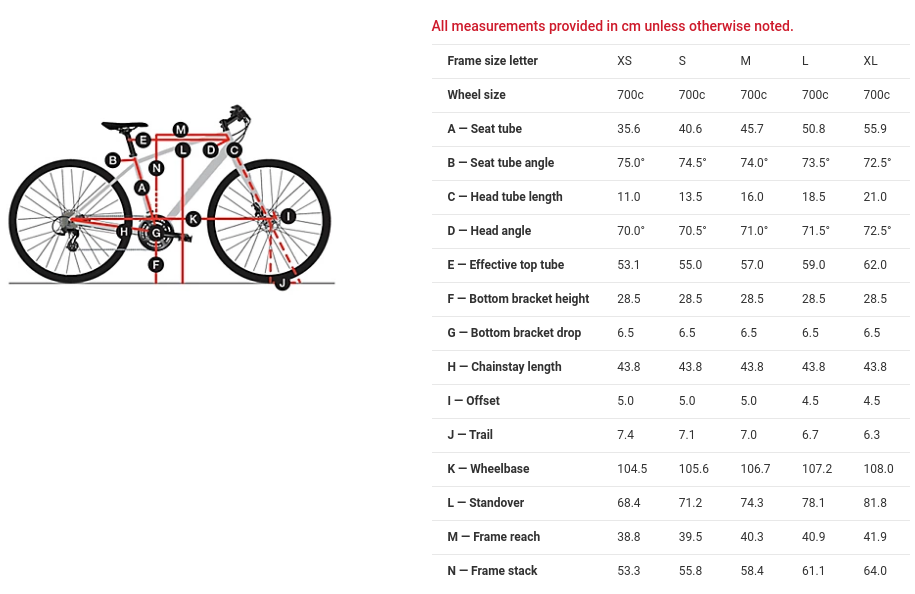
\includegraphics[width=\linewidth]{trek_fx_sport_4_geo}%
\label{fig:trek_fx_sport_4_geo}
\caption{}
\end{subfigure}
\end{figure}
As an example, we will compare two same bikes, but with different sizes. In each case we are assuming that the 
rider's centre of mass will be in the same height and that he is decelerating at $-3\frac{m}{s^2}$. The bike used 
for our demonstration is TREK FX Sport 4 (fig.~\ref{fig:trek_fx_sport_4}), which is a fully rigid fitness bicycle.
\end{document}
